\documentclass[10pt,addpoints]{exam}
\usepackage[utf8]{inputenc}
\usepackage[spanish,es-noshorthands]{babel}
\usepackage{hyperref}
\usepackage{amsmath}
\usepackage{amsfonts}
\usepackage{amssymb}
\usepackage{graphicx}
\usepackage{tikz}
\usepackage{multicol}
\usepackage[papersize={6.5in,8.5in},width=5.5in,height=7.5in]{geometry}
%\printanswers
\begin{document}
\title{\begin{minipage}{.2\textwidth}
        
\includegraphics[height=1.75cm]{Images/logo-colegio.png}
       \end{minipage}
\begin{minipage}{.55\textwidth}
 \begin{center}
Prepar\'andonos - Prueba Saber 11 \\Matem\'aticas $11^{\circ}$
\end{center}
\end{minipage}
\begin{minipage}{.2\textwidth}

\includegraphics[height=1.75cm]{Images/logo-sed.png} 
\end{minipage}
}
\author{Germ\'{a}n Avendaño Ram\'{i}rez\thanks{Lic. Mat. U.D., M.Sc. U.N.}}
\date{}
\maketitle
\begin{center}
\fbox{\fbox{\parbox{5.5in}{\centering
Instrucciones: Responda las preguntas siguientes, justificando cada respuesta.}}}
\end{center}
\vspace{0.1in}
\makebox[\textwidth]{Nombres: \hrulefill, curso:\underline{\hspace{48pt}}, fecha:\underline{\hspace{3cm}}}
\begin{questions}
\question
Si $a$, $b$ y $c$ son números primos diferentes y $n=\dfrac{a^{-1}b^{-3}}{a^{-2}b^{-4}c^{-2}}$, es correcto afirmar que
\begin{choices}
\begin{multicols}{2}
 \CorrectChoice $n$ es entero
 \choice $n$ es primo
 \choice $n$ es un racional negativo
 \choice $n$ es irracional
\end{multicols}
\end{choices}
\question Un almacén distribuye computadores de dos marcas (1 y 2). Durante el mes de diciembre uno de sus vendedores vendió 60 computadores. Por cada tres computadores de la marca 1 vendió dos de la marca 2. Si recibió una comisión de \$10\,000 por cada computador de la marca 1 y una comisión de \$20\,000 por cada computador de la marca 2, la comisión total que recibió en el mes de diciembre fue

\begin{oneparchoices}
  \choice \$60\,000
  \choice \$120\,000
  \CorrectChoice \$840\,000
  \choice \$720\,000
\end{oneparchoices}
\question En una empresa el costo de producir un computador es $c$. Si se venden $y$ computadores con un precio de $v$ cada uno, entonces la expresión correcta para la ganancia $g$ es
 \begin{choices}
  \begin{multicols}{2}
   \choice $g=y(v+c)$
   \choice $g=vy-c$
   \choice $g=c-vy$
   \CorrectChoice $g=y(v-c)$
  \end{multicols}
 \end{choices}
\question Considere las siguientes proposiciones relacionadas con soluciones de ecuaciones:
\begin{enumerate}
 \item[(1)] La ecuación $\dfrac{1+2x}{1+x}=\dfrac{x}{1+x}$ \textbf{no} tiene solución en el conjunto de los números reales.
 \item[(2)] La ecuación $\sqrt{x^{2}-9}=4$ tiene exactamente 2 soluciones reales. 
\end{enumerate}
De las proposiciones es correcto afirmar que
\begin{choices}
 \begin{multicols}{2}
  \choice (1) es verdadera, (2) es falsa
  \choice (1) y (2) son falsas
  \choice (1) y (2) son verdaderas
  \CorrectChoice (2) es verdadera y (1) es falsa
 \end{multicols}
\end{choices}
\question Considere las siguientes proposiciones:
\begin{enumerate}
 \item[(1)] Las diagonales de un cuadrilátero pueden ser perpendiculares.
 \item[(2)] Un cuadrilátero puede tener todos sus ángulos obtusos. 
\end{enumerate}
De las proposiciones es correcto afirmar que:
\begin{choices}
 \begin{multicols}{2}
  \CorrectChoice (1) es verdadera, (2) es falsa
  \choice (1) y (2) son verdaderas
  \choice (1) y (2) son falsas
  \choice (1) es falsa, (2) es verdadera
 \end{multicols}
\end{choices}
\question Sean $PQR$ y $STU$ dos triángulos tales que el ángulo en $Q$ es congruente con el ángulo en $T$. Una condición suficiente para que los triángulos sean semejantes es

\begin{oneparchoices}
  \choice $\dfrac{PR}{SU}=\dfrac{QR}{TU}$
  \CorrectChoice $\dfrac{PQ}{ST}=\dfrac{QR}{TU}$
  \choice $\dfrac{PQ}{ST}=\dfrac{PR}{SU}$
  \choice $\dfrac{PR}{TU}=\dfrac{QR}{SU}$
\end{oneparchoices}
\question De las gráficas de las funciones definidas por $f(x)=4(x-1)^{2}+3$ y $g(x)=4(x+1)^{2}+3$ es correcto afirmar que
\begin{choices}
  \choice tienen el mismo vértice
  \choice una es abierta hacia arriba y la otra es abierta hacia abajo
  \CorrectChoice se cortan en un punto
  \choice las dos tienen puntos de corte con el eje $x$
\end{choices}
\question Un caficultor que exporta la misma cantidad de café durante los meses 1, 2 y 3 recibe su pago en pesos colombianos.
\begin{center}
 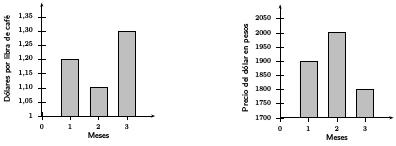
\includegraphics{./Images/cafe.jpg}
 % cafe.jpg: 0x0 pixel, 300dpi, 0.00x0.00 cm, bb=
\end{center}
Teniendo en cuenta los gráficos, es correcto afirma que recibe
\begin{choices}
 \choice más pesos en el mes 1
 \choice más pesos en el mes 2
 \choice la misma cantidad de pesos los tres meses
 \CorrectChoice más pesos en el mes 3
\end{choices}

%\answerline
\end{questions}
%cuadro de puntajes
%\begin{center}
%\gradetable[h][pages]
%\end{center}
\end{document}